% R. Richiesta modifica. Il titolo é troppo ampio e forse anche errato (qui sei ancora alla fase di definizione dei requisiti che abbiamo fatto rientrare in engineering, mentre il design da come raccontato nel capitolo 2 corrisponde piú alla concettualizzazione). Provo a modificare (qualche riserva).
% \chapter{Ontology design}
\chapter{The Prompt Engineering Ontology: Requirements Specification}
% R. Spiegazione modifica. Richiamato il nome dell'ontologia. Modificata la parte finale della frase, è ovvio che è stata scelta secondo delle motivazioni. Rimosso \\. Introdotto subito LOT.
% This chapter details the design phase of the prompt engineering ontology, starting from an ontology engineering methodology chosen based on specific motivations.\\
This chapter details the design phase of the \textit{Prompt Engineering Ontology} PEO, based on LOT, a state-of-the-art ontology engineering methodology.
% R. Spiegazione modifica. Inutile.
% In the background chapter, in particular in the sections \textit{"Ontology engineering methodologies"} and \textit{"LOT methodologies"} the main state-of-art ontology engineering methodologies have been illustrated:
% \begin{itemize}
%     \item \textbf{Methontology}
%     \item \textbf{NeOn}
%     \item \textbf{eXtreme design}
%     \item \textbf{LOT - Linked Open Terms}
% \end{itemize}
% Additionally, in the section \textit{"Ontology engineering using large language models"} two experimental methodologies were analysed, including \textbf{NeOnGPT}, which employs large language models. Each methodology has its features and defines a workflow in order to develop successfully an ontology. The choice of the methodology to follow during the design and development phase is based on an analysis of the pros and cons of each, considering not only their features but also the available resources and the related projects provided by each one. \\

% R. Spiegazione modifica. Ho anticipato sopra che usi LOT. Questo paragrafo è dedicato alle motivazioni.
% In the state-of-the-art study, the most recent and comprehensive methodology is the \textbf{LOT methodology}, which I have decided to choose and according to which the development of the prompt engineering ontology will be carried out.
Compared to other methodologies analysed, LOT is a recent methodology, introduced in 2022, and has been used in various projects such as the 'Ciudades Abiertas' project \cite{ciudad} for the construction of a set of ontologies used for sharing open data, and the BIMERR project \cite{bimerr}, in which ontologies for sustainable construction were developed \cite{bountouni2021bimerr}, among many others available on the LOT methodology website: \href{https://lot.linkeddata.es/}{https://lot.linkeddata.es/}.
% R. Richiesta modifica. Usare il riferimento al capitolo.
% LOT has not only been successfully applied in industrial projects, but also in the development of various research ontologies, as seen in the background chapter, as it provides a straightforward and iterative method for designing and developing ontologies.
LOT has not only been successfully applied in industrial projects, but also in the development of various research ontologies, as seen in Chapter~\ref{chapter:background}, as it provides a straightforward and iterative method for designing and developing ontologies.
Another reason for choosing LOT is its ease of learning, as it is inspired by the agile methodology in software development. The Linked Open Terms project not only provides very useful examples of ontologies to draw inspiration. LOT offers a Github repository \cite{lot_github} with all the necessary resources to be used in the specification of requirements.
% R. Richiesta modifica. Scrivere meglio. Magari dividere la frase. Prendi spunto delle innumerovoli modifiche linguistiche nel capitolo 2. Curare la scrittura perchè denota completa mancanza di cura e interesse per quello che hai fatto e indispone chi legge. fatto
This last aspect is very important because the main drawback of the other methodologies analysed is the lack of concrete guidelines and the relevant tools to use, tools that, when mentioned, are often obsolete or inaccessible.
This complicates the work of a developer who is approaching ontology engineering for the first time, as he needs to understand the fundamentals of the methodology but also figures out which development, validation, and testing software to use.
The LOT methodology, thanks not only to the numerous available resources but also to the clear and precise description of the method and the recent tools to be used, resolves these issues and simplifies the developer's work.
The LOT methodology has an inherently iterative nature and is oriented towards the publication of ontologies according to the FAIR principles \cite{fair_eu}, including specific recommendations, tips and potential
tools that can be helpful to ontology developers.
Moreover, the methodology extends the state-of-art methodologies like \textit{NeOn} and \textit{Methontology} with a modern approach.

The LOT methodology was preferred over recently introduced techniques that involve the use of LLMs.
Although these techniques automate the process, they are computationally expensive and require numerous checks to verify the syntactic and semantic correctness of the produced artifact.
Another downside is the lack of actual ontology projects implemented using LLMs, as these are very recent techniques that have not been tested on real projects but only on experimental cases.
% R. Richiesta modifica. Usare il riferimento al capitolo background (come mostrato in un commento precedente in questo capitolo). fatto
In the following sections, the application of the LOT methodology, methodology that has been discussed in Chapter \ref{chapter:background}, to the design and implementation of PEO will be described, following the workflow outlined and described in the background chapter.

% \section{Ontology requirements specification}
\section{Use Case Specification}
The LOT methodology includes six mandatory phases (plus one optional) in the ontology requirements specification.
% R. Richiesta modifica. Referenziare correttamente la figura. fatto
At the end of each phase, a document is produced containing the analysed aspect of the specifications, as shown in the following figure \ref{fig:13}:
\begin{figure}[H]
    \centering
    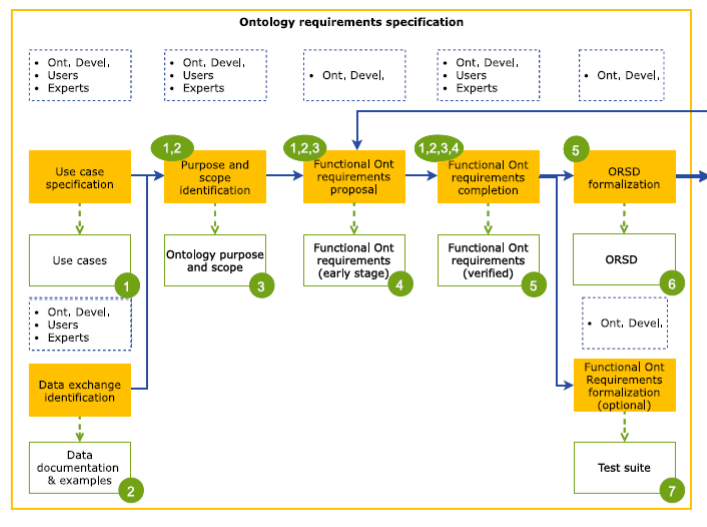
\includegraphics[width=0.9\linewidth]{Figures/fig_13.PNG}
    \caption{Ontology requirements specification workflow}
    \label{fig:13}
\end{figure}
In detail the phases are the following:
\begin{enumerate}
    \item Use case specification
    \item Data exchange identification
    \item Purpose and scope identification
    \item Functional ontology requirements proposal
    \item Functional ontology requirements completion
    \item ORSD formalization 
    \item Functional ontology requirements formalization (optional)
\end{enumerate}

% R. Richiesta modifica. Questa dovrebbe essere una subsection. fatto. R. rimosso titolo perché é l'unica subsection della section.
% \subsection{Use case specification}
The first step in the design of PEO is the use case specification, this phase involves domain experts, ontology developers and users and it has the goal to imagine and specify how the ontology can be used in real life by real users.
% R. Richiesta modifica. Sistemare la punteggiatura ed evitare 'I' 
Taking into account the domain, the possible use and the possible users we decided to specify ten use cases.
Each use case has a name, a description, a list of actors and a flow.

% R. Richiesta modifica. Le sezioni use case x dovrebbero tutte essere subsubsection o forse evitare proprio che siano titoli.
\paragraph{Use case 1}
% R. Richiesta modifica. Mettere in bold o in corsivo il nome dell'item (name, description, ...) fatto
\begin{itemize}
    \item \textit{Name:} Optimizing LLM Responses
    % R. Richiesta modifica. La O in PEO sta per "ontology" quindi dire "the PEO ontology" equivale a dire "the Prompt Engineering Ontology ontology". Rimuovere ontology. Controllare tutte le occorrenze. fatto
    \item \textit{Description:} Researchers use PEO to design optimized prompts that improve LLM response quality.
    \item \textit{Actors:} Researcher, PEO, LLM.
    \item \textit{Flow:} The researcher uses the ontology to identify appropriate prompts for different types of tasks creating a set of selected prompts. Selected prompts are given as input to the LLM and responses are evaluated according to specific metrics on consistency, completeness and quality decided by the researcher.
\end{itemize}
% R. Richiesta modifica. Mi pare abbastanza ripetitivo. Potresti integrare nell'elenco puntato le poche informazioni in più che da il paragrafo successivo.
\paragraph{Use case 2}
\begin{itemize}
    \item \textit{Name:} Bias analysis
    \item \textit{Description:} Researchers use PEO to generate responses and detect bias in the considered LLMs.
    \item \textit{Actors:} Researcher, PEO, LLMs
    \item \textit{Flow:} The researcher uses the ontology to generate prompts on sensitive topics (e.g., gender, ethnicity) and prompts are tested on one or more LLMs. Responses are collected using bias and fairness metrics and results are collected in order to improve prompts and considered models. 
\end{itemize}
% R. Richiesta modifica. Mi pare abbastanza ripetitivo. Potresti integrare nell'elenco puntato le poche informazioni in più che dail paragrafo successivo. Stessa considerazione dovrebbe valere in generale per tutti gli use case. Ovviamente, controlla prima se è così caso per caso e valuta se applicare il suggerimento.

\paragraph{Use case 3}
\begin{itemize}
    \item \textit{Name:} Code generation
    \item \textit{Description:} Developers use prompt engineering techniques applied to a chosen LLM to generate source code in a specific programming language for a specific task.
    \item \textit{Actors:} Developers, PEO, LLM
    \item \textit{Flow:} The developer is working on an Android application written in Java and needs code to control the actions on a button. Using the ontology, he chooses the most appropriate prompt engineering technique and applies it to the creation of the prompt to a large language model of his choice,  resulting in Java code as output. The code is tested and integrated into the application. 
\end{itemize}

\paragraph{Use case 4}
\begin{itemize}
    \item \textit{Name:} Prompt engineering lesson
    \item \textit{Description:} The teacher uses PEO to teach prompt engineering techniques exploring different techniques and prompt described.
    \item \textit{Actors:} Teacher, students, PEO. 
    \item \textit{Flow:} The teacher opens the ontology and shows with proper explanation different prompt engineering techniques represented in the ontology.
\end{itemize}
% R. Spiegazione modifica. Rimossa perchè vaga e ridondante
% The prompt engineering ontology can be used for learning prompt engineering techniques, thanks to the classes and relations present, and serves as a valuable support for a computer science instructor during lessons.

\paragraph{Use case 5}
\begin{itemize}
    \item \textit{Name:} LLMs lesson
    \item \textit{Description:} The teacher uses PEO to teach the different LLMs available.
    \item \textit{Actors:} Teacher, students, PEO.
    \item \textit{Flow:} The teacher opens the ontology and shows with proper explanation different LLMs represented in the ontology. 
\end{itemize}
% R. Spiegazione modifica. Rimossa perchè vaga e ridondante
% Similar to the previous use case, the ontology of prompt engineering represents state-of-the-art large language models and their relations. This representation can be useful for an instructor to explain large language models during lessons.
% SG ok chiaro
\paragraph{Use case 6}
\begin{itemize}
    \item \textit{Name:} Social media content creation
    \item \textit{Description:} The content creator uses PEO to generate prompts that optimize the creation of articles, social media posts and other textual content.
    \item \textit{Actors:}  Content creator, PEO, LLM
    \item \textit{Flow:} The content creator opens the ontology and chooses the appropriate technique in order to generate text for a post on social media using a specific large language model. The content creator adapts the response according to his target.
\end{itemize}



\paragraph{Use case 7}
\begin{itemize}
    \item \textit{Name:} Image generation
    \item \textit{Description:} The content creator uses PEO to create a prompt to be given as input to a specific large language model capable of generating an image.
    \item \textit{Actors:} Content creator, PEO, LLM.
    \item \textit{Flow:} The content creator wants to create an AI-generated image for a video and he uses the ontology to choose the best large language models able to generate image, he chooses the prompt engineering technique to create the prompt in order to generate image. He watches the output and he continues to use the ontology to generate prompts in order to refine the image.
\end{itemize}

\paragraph{Use case 8}
\begin{itemize}
    \item \textit{Name:} Prompt engineering experiments
    \item \textit{Description:} Students use PEO to explore and create effective prompts to improve language model responses.
    \item \textit{Actors:} Students, PEO, LLM.
    \item \textit{Flow:} Students explore the ontology in order to understand different prompting techniques applying them to a chosen large language model.
\end{itemize}

\paragraph{Use case 9}
\begin{itemize}
    \item \textit{Name:} Large language models learning
    \item \textit{Description:} Students use PEO to learn different types of large language models.
    \item \textit{Actors:} Students, PEO
    \item \textit{Flow:} Students explore different large language models represented in the ontology and the relations among them, learning all the features of each large language model.
\end{itemize}

\paragraph{Use case 10}
\begin{itemize}
    \item \textit{Name:} Explanation computer science topics
    \item \textit{Description:} Student wants to generate a prompt using PEO in order to explain a computer science topic.
    \item \textit{Actors:} Student, PEO, LLM
    \item \textit{Flow:} The student uses the ontology to choose the most appropriate prompt engineering technique in order to generate using large language models. The student reads the obtained LLM response and can create a new prompt using another technique represented in the ontology.
\end{itemize}

\section{Data Exchange Identification}
The goal of the data exchange identification activity is to provide the necessary documentation about the domain to be modelled.
Essentially, this phase involves gathering heterogeneous sources of information, such as scientific papers, websites, datasets, and similar existing ontologies.
% R. semplificato.
% The LOT methodology does not provide a clear indication of how to represent this documentation, so for simplicity and clarity, I have decided to collect the links to the scientific papers and web pages containing information to be represented in the ontology in a dedicated file.
Since LOT does not provide a clear indication on how to represent this documentation, we simply noted the URLs of the gathered resources.
% The list of papers chosen as a source for the prompt engineering ontology is as follows:
% R. Richiesta modifica. Aggiungere i criteri. Per esempio, potrebbero essere i più recenti, i più citati, i piú completi. Si potrebbe fare anche qualche considerazione sul dove sono pubblicati. Ricordo che per i paper di prompt engineering avevo abbozzato alcune moticazione nel file dei riferimenti. Potrebbe esserci qualcosa di utile.
The following list of papers was chosen as a source for PEO:

\begin{itemize}
\item A Systematic Survey of Prompt Engineering in Large Language Models: Techniques and Applications \cite{sahoo2024systematic}

\item Pre-train, Prompt, and Predict: A Systematic Survey of Prompting Methods in Natural Language Processing \cite{liu2023pre}

\item A Survey of Large Language Models \cite{zhao2023survey}

\item Investigating Prompt Engineering in Diffusion
Models \cite{witteveen2022investigating}

\item A Survey on Large Language Models: Applications,
Challenges, Limitations, and Practical Usage \cite{hadi2023survey}

\item Large Language Models: A Survey \cite{minaee2024large}
\end{itemize}
% R. Richiesta modifica. Aggiungere i criteri.
The list of website chosen is the following:
\begin{itemize}
    \item \href{https://www.promptingguide.ai/}{Prompting Guide}
    
    \item \href{https://github.com/Hannibal046/Awesome-LLM}{Awesome-LLM}

    \item \href{https://llmmodels.org/}{List of LLMs}

    \item \href{https://learnprompting.org/}{Learn prompting}
\end{itemize}
Unfortunately, the resources found and deemed useful for developing the ontology are not many, as the topic is very recent.
Additionally, no datasets containing prompts generated with specific techniques were found.
In contrast, only datasets with generic prompts for text generation, such as the dataset available on Huggingface, "awesome-gpt-prompts" \cite{awesome_gpt}, and the "diffusion-db" dataset \cite{diffusion_db}, which, although it contains over 16 million prompts for image generation, does not specify the prompt engineering technique used.

\section{Purpose and Scope Identification}
% R. Richiesta modifica. Frase scritta male (per esempio "in this phase there is" non mi sembra grammaticalmente corretto) e troppo lunga. Usare la punteggiatura. Ho fatto diverse modifiche simili in capitolo 2. Ora dovrebbe essere chiaro come puoi farle tu.
From use cases and the domain documentation provided in the data exchange identification task, in this phase there is the specification of the purpose: what is the objective of PEO and the specification of the scope of the ontology: what it is going to be represented in the ontology.
% Spiegazione modifica. Richiamato il termine objective usato nella frase precedente.
% PEO aims to formalize knowledge about the creation and various types of prompts for the different LLMs available by making it accessible to both experienced and less experienced users.
The objective of PEO is to formalize knowledge about the creation and various types of prompts for the different LLMs available by making it accessible to both experienced and less experienced users.
% R. Spiegazione modifica. Ridondante.
% This is the purpose of the PEO.
% R. Spiegazione modifica. Presente indicativo. Richiamato il termine scope.
% PEO is going to cover:
PEO aims at covering the following scope:
\begin{itemize}
    \item LLMs available to users
    \item Prompt engineering techniques
    \item Task that can be solved using a LLM
    \item Examples of prompts specific to the LLM
\end{itemize}
% R. Spiegazione modifica. Ridondante.
% This is the scope of the PEO.
In general, the goal of the project and the ontology is to create a resource accessible to everyone on a recently introduced topic, for which there are not many available resources.
This resource aims to support not only the learning but also the application of prompt engineering techniques and LLMs.

\section{Functional ontology requirements specification}
% R. Richiesta modifica. La prima parte della frase non si capisce (forse perché grammaticalmente errrata)
In LOT methodology there are three possible ways to specify the requirements: CQs, natural language statements and tabular information containing concepts, relations, and attributes.
% R. Richiesta modifica. Usare il riferimento al capitolo
% As seen in the background chapter, competency questions are widely used in ontology engineering and allow for clearly expressing the functional requirements of an ontology.
As seen in Chapter~\ref{chapter:background}, competency questions are widely used in ontology engineering and allow for clearly expressing the functional requirements of an ontology.
In the case of PEO, based on the use cases and the purpose and scope identification described earlier, we have identified sixteen CQs:
\begin{itemize}
    \item \textbf{CQ1:} What is prompt engineering?

    \item \textbf{CQ2:} What is a prompt?

    \item \textbf{CQ3:} What are prompting techniques?

    \item \textbf{CQ4:} What are image prompting techniques?

    \item \textbf{CQ5:} What are code prompting techniques?

    \item \textbf{CQ6:} Which task does a prompt solve?

    \item \textbf{CQ7:} Which prompts are generated using a prompting technique?

    \item \textbf{CQ8:} What are the responses that follow each prompt?

    \item \textbf{CQ9:} What are possible tasks?

    \item \textbf{CQ10:} Which tasks are related to the text?

    \item \textbf{CQ11:} What is a chat?

    \item \textbf{CQ12:} What is a large language model?

    \item \textbf{CQ13:} What types of large language models are available?

    \item \textbf{CQ14:} What are large language models architectures?

    \item \textbf{CQ15:} What are large language models capabilities?

    \item \textbf{CQ16:} What companies develop large language models?
\end{itemize}

% R. Richiesta modifica. Usare la footnote per il link.
CQs are saved into an excel file, the template is available in the official Github repository \footnote{https://github.com/oeg-upm/LOT-resources}.
The Excel file not only contains the CQs, but also specifies for each one: the identifier, the domain, the answer, the status (Proposed, Accepted, Rejected, Pending, Deprecated), comments, and priority (high, medium, and low).
All the CQs have a high priority, as they form the foundation of PEO, covering both prompt engineering and LLMs.

\section{Document Formalization}
% R. IMPORTANTE. Richiesta modifica. Dall'inizio di questa sezione fino a "In writing the ORSD for PEO" stai discutendo dei basics e non un tuo contributo. Spostare nel capitolo 2. Inoltre, hai mischiato LOT e Neon in questo paragrafo, dividi le informazioni che riguardano Neon (e le metit nella sezione su Neon) e quelle che riguardano LOT (e le metti nella sezione su LOT). Dopo se hai bisogno di metterle esplicitamente a confronto puoi farlo in LOT.
The final step in the specification of ontology requirements is the writing of the ORSD, a document that gathers the main information defined in the previous phase, namely the purpose and scope of the ontology, the use cases, the functional requirements (expressed through CQs), and the non-functional requirements.
% R. Richiesta modifica. Usare il riferimento al capitolo ed evitare 'I'.
First introduced by the NeOn methodology, which we discussed in the previous chapter, the writing of the ORSD follows a specific sequence of tasks to ensure its correctness and completeness.
% R. Spiegazione modifica. Rimosso il titolo dell'articolo citato.
% The workflow is described in the paper \textit{How to Write and Use the Ontology Requirements Specification Document}\cite{suarez2009write} and involves a sequence of eight tasks, starting from ontological needs: 
The workflow \cite{suarez2009write} involves a sequence of eight tasks, starting from ontological needs: 
\begin{enumerate}
    \item Identify purpose, scope and implementation language.
    \item Identify intended end-users
    \item Identify intended uses
    \item Identify requirements
    \item Group requirements
    \item Validate the set of requirements
    \item Prioritize requirements
    \item Extract terminology and its frequency
\end{enumerate}

% R. Spiegazione modifica. Semplificato. Cambiato al presente indicativo.
% The LOT methodology adopted the ORSD introduced by NeOn but adapted it with appropriate modifications.
LOT adopts (a customized version of) the ORSD introduced by NeOn.
Unlike NeOn, it does not consider the "user" field as mandatory, and the glossary of terms is built starting from the competency questions.
% R. Richiesta modifica. Usare la footnore per il link.
In writing the ORSD for PEO, the  template from the official LOT repository \footnote{https://github.com/oeg-upm/LOT-resources/tree/master/templates\%20for\%20ORSD} was used. 
In the document, the information obtained in the previous phases has been included, namely purpose and scope identification and ontology requirements in the form of CQs.
Additionally, further information that emerged during the requirements gathering phase has also been included:
\begin{itemize}
    \item Implementation language 
    \item Intended End-Users 
    \item Intended Uses
    \item Non-Functional Requirements
\end{itemize}
In detail, the implementation language is OWL using the Protegé software\cite{protege_sw}, an open-source popular software released by Stanford University.
As seen in the use cases, the intended end-users of PEO are:
\begin{itemize}
    \item Researchers in the field of AI using LLMs for research purpose.
    \item Software engineers and developers.
    \item Educators and trainers teaching students or professionals about AI and prompt engineering, using the ontology as a learning and instructional tool.
    \item Content Creators using LLMs for generating content.
    \item Undergraduate and high school students learning about AI, LLMs and prompt engineering, using the ontology to understand core concepts and experiment with language models.
\end{itemize}
Starting from the use cases, it is possible to easily deduce the intended uses:
\begin{itemize}
    \item Prompt generation
    \item LLMs learning
    \item Prompt engineering learning
    \item Prompt generation for a specific task
\end{itemize}
% R. Richiesta modifica. Rimuoverei il primo requisito per diverse ragioni: 1) non misuri la semplicitá/usabilitá, quindi non dai un'indicazione sull'averlo soddisfatto o meno, 2) é esposto in maniera vaga, facile da usare puó riferirsi a svariate cose tra cui la comprensibilitá dei nomi dei costrutti,  le modalitá di accesso (che per il momento é SPARQL che non é la cosa piú facile del mondo), la presenza o meno di una GUI (per il momento no), la comprensibilitá dei ragionamenti, ecc.
% R. Richiesta modifica. NFR2, NFR3 e NFR6 non mi sembrano requisiti non funzionali, riguardano il contenuto.
% R. Richiesta modifica. Aggiungere come requisito non funzionale che é accessibile sui principali repository di ontologie (puoi mostrare nelle sezioni successive che l'hai effettivamente fatto).
Regarding non-functional requirements, i.e., the characteristics, qualities and general aspects not related to the ontology content that the ontology should satisfy, we have identified three non-functional requirements:
\begin{itemize}
    \item \textbf{NFR1:} The ontology must be published on main ontology repositories
    \item \textbf{NFR2:} The ontology must have exhaustive documentation.
    \item \textbf{NFR3:} The ontology must be easy to update.
\end{itemize}
% R. Richiesta modifica. Modificare il paragrafo seguente in base alle modifiche dei requisiti. fatto
Those non-functional requirements match with the desired properties of PEO, since the ontology has to be accessible for everyone by publishing on main ontology repositories. The documentation  must be exhaustive and clear for users to understand the content of the ontology and it could be useful for possible updates.




